\section{Direct SYS clock-loss capture after SPI}
A temporary PM SRAM diagnostic recorded the SPI inputs, fixed SYS MMCM LOCK, CAP MMCM LOCK and SYS reset on a clock independent of SYS. It survived SYS reset. One idle control and five signature reads yielded two captured reset events (after reads1 and0). Every transmitted frame contains64sampled SCK transitions. No output release or card-direction change occurred, and no UART/PLL command was sent during these captures.

In both events fixed SYS MMCM LOCK drops and SYS reset asserts. CAP MMCM LOCK remains high. Fixed LOCK returns and SYS reset releases two watch-clock ticks later. This directly establishes the clock-domain reset path; it does not establish a FIN defect, MCU action, or external PLL failure. Narrower input glitches can be missed.

The watch clock is approximately SYS frequency (nominal40.0787MHz), despite120MHz source/CSR metadata. This follows independently from the idle watch/SYS counter ratio and200watch ticks per600Kasli-tick SPI half-cycle. This is not counter calibration. With that nominal scale the recorded LOCK-low intervals are8.483/8.508us, after9.826/9.513ms of running watch time from HSEL deassertion. A simultaneous stop of watch and MGT clocks is not represented in those times. Clock input assumptions need separate audit before rated-throughput or absolute timing qualification; no CDCE output settings were changed.

The DIO schematic identifies FIN1101K8X repeaters and100ohm terminations on both sides. Open-circuit fail-safe is not proof of a defined disconnected-but-terminated input. Correct3.3V supply alone is not a CMOS/LVDS mismatch. Oscilloscope observation at the FIN/HDMI path and MGT clock is still needed to identify the electrical cause.

Exact golden c7c42d28 SRAM was restored and physical ADC, stable SYS and PGOOD checked. Kasli SPI remains driven at idle0 with slot6mask0x00b0. Existing campaign case statuses remain unchanged. Raw records, HDL, simulation, source/bit archive and checksum qualification are retained in system/evidence-clock-observer-20261113.

\begin{figure}[htbp]\centering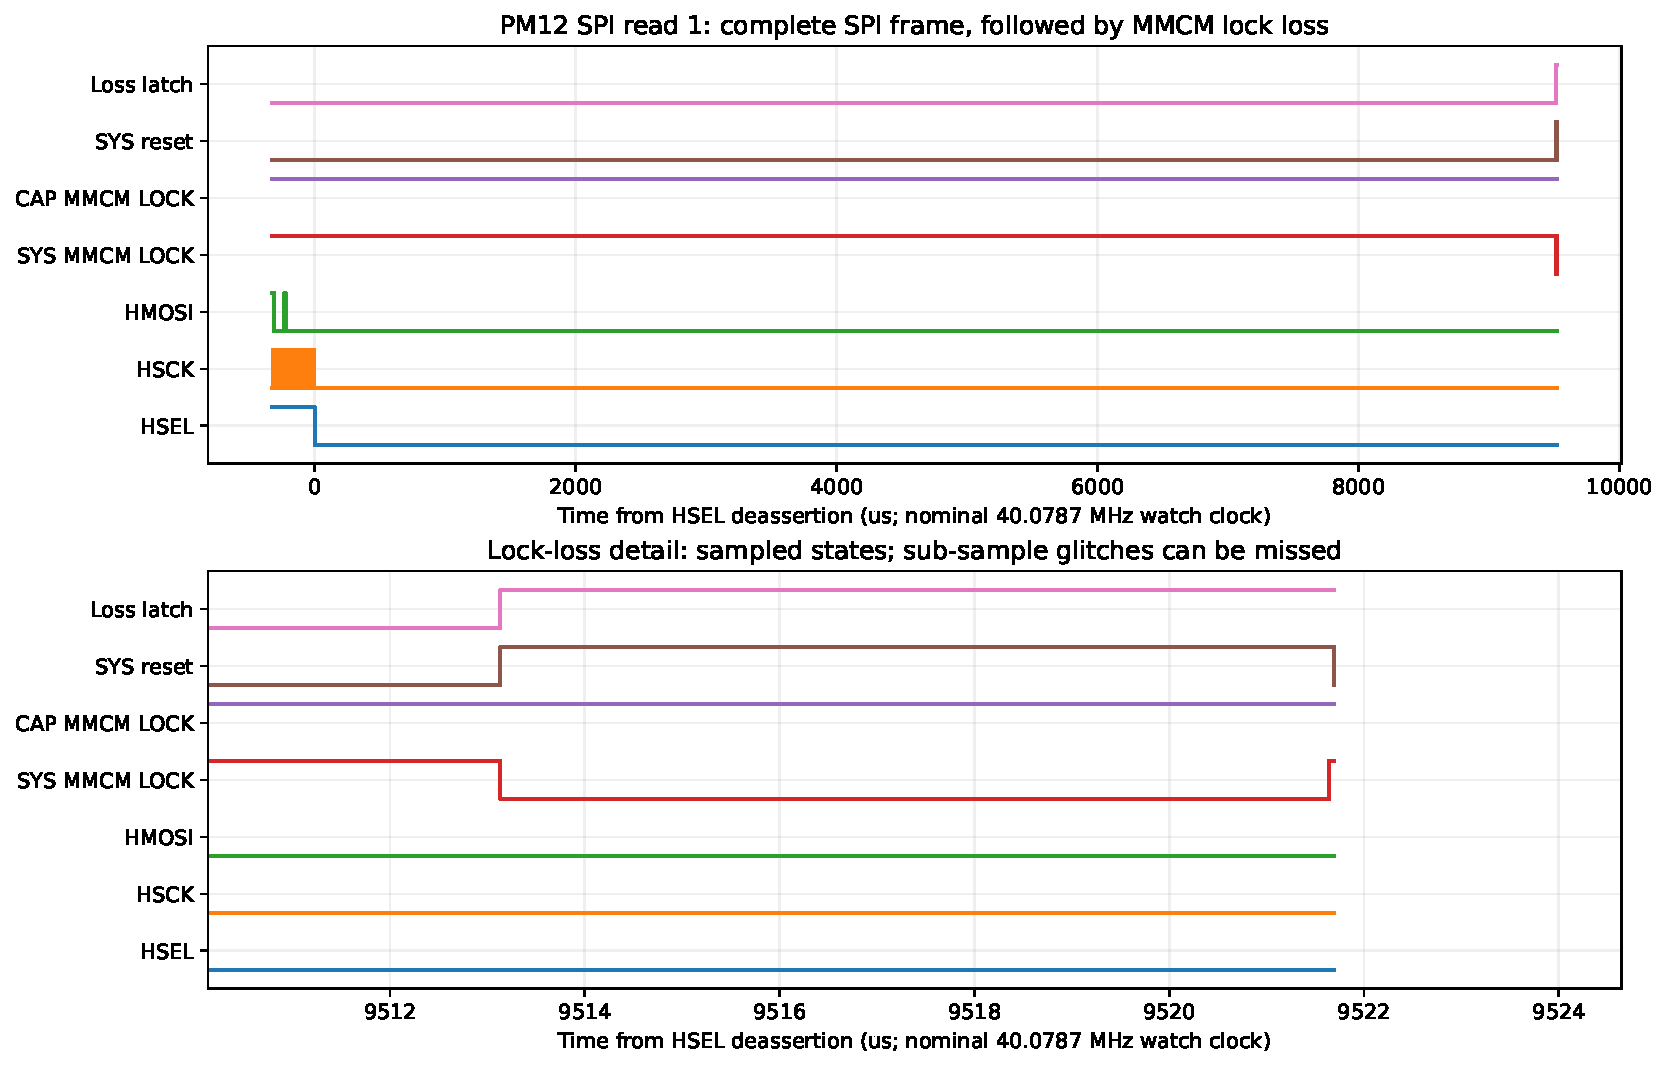
\includegraphics[width=\textwidth]{clock-loss-read1.pdf}\caption{SPI read1 and later SYS MMCM lock loss. Time scale assumes a continuously running40.0787MHz observation clock.}\end{figure}
\begin{figure}[htbp]\centering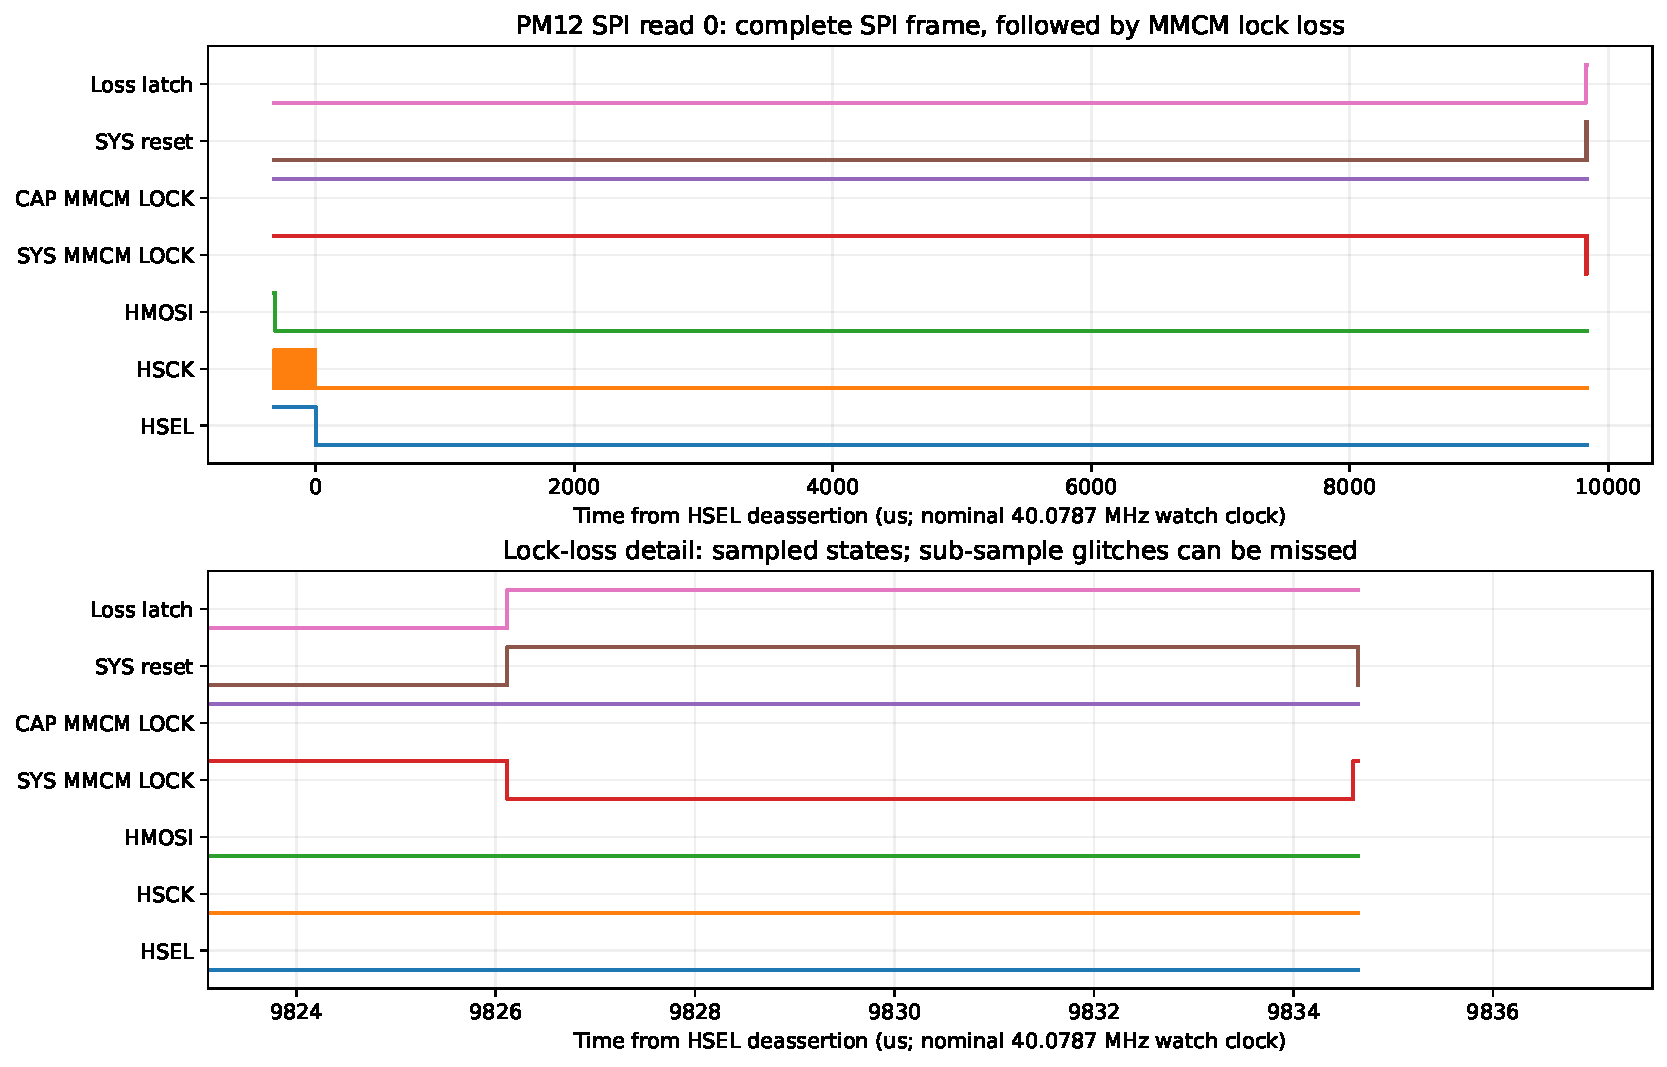
\includegraphics[width=\textwidth]{clock-loss-read0.pdf}\caption{Independent repeat after SPI read0. No release of Kasli outputs occurs.}\end{figure}
\clearpage
